
\begin{flushleft}
	\begin{itemize}
		
		\item So far, we put all of our code in the \textbf{main() method}. 
		\item \textbf{That’s not exactly object-oriented}. 
		\item Leave the procedural world behind, get the out of main(), and start making some objects of our own. 
		\item We’ll look at what makes object-oriented (OO) development in Java so much fun. 
		\item Let’s understand this with a use-case:  \\
		Creat a Shape Application with below requirement:
		
		\newimage{0.5}{content/chapter0/images/new16.png}
		
		\item For this, Raj followed Procedure-Oriented approach while Ram followed Object-Oriented approach to develop the code.
		
		\newpage
		\tabletwo{
			\hline
			Raj's Procedure-Oriented approach & Ram's Object-Oriented approach  \\
			\hline
			\bigskip \bigskip
			\codeblock{
				rotate(shapeNum) \{ \\
				\s	//code here \\
				\} \\
				playSound(shapeNum) \{ \\
				\s	//code here \\
				\} 
			} & \bigskip 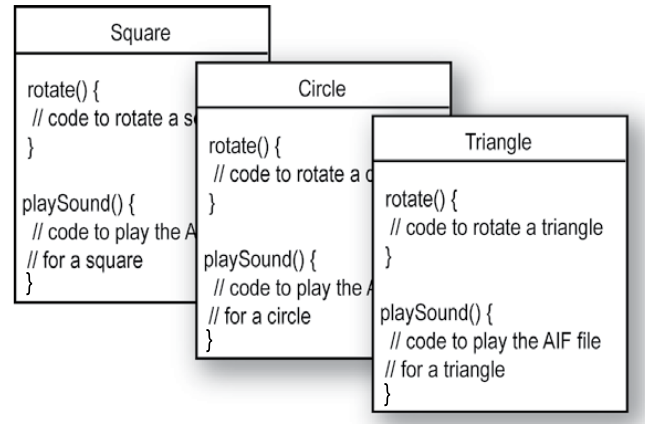
\includegraphics[scale=0.3]{content/chapter0/images/new17.png}  \\
			\hline
		}
		
		\item But wait! There’s been a spec change.
		
		\newimage{0.35}{content/chapter0/images/new18.png}
		
		\item In order to reflect the new requirements, here's what Raj and Ram decided to do:
		
		\newpage
		
		\tabletwo{
			\hline
			Back in Raj's cube  & At Ram's laptop in a cafe  \\
			\hline
			Raj will need to make changes in existing code and perform the testing again:
			\bigskip
			\codeblock{
				\color{red}
				rotate(shapeNum) \{ \\
					//new changes to add amoeba \\
				\} \\
				playsound(shapeNum) \{ \\
					//add change for amoeba \\
				\} 
			} & 
			Ram just need to create one more class called "Amoeba":
			 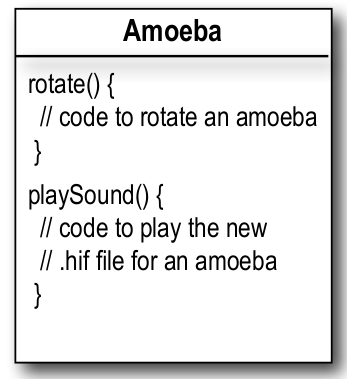
\includegraphics[scale=0.5]{content/chapter0/images/new19.png}  \\
			\hline
		}
	\end{itemize}

	\quest{So what do you like about OO?}{
		\begin{itemize}
			\item Design software as per real world usage.
			\item New changes can be incorported easily.
			\item Not messing around with code already tested, just to add a new feature.
			\item Data \& methods that operate on that data are together in one class.
			\item Code can be re-used in other applications.
		\end{itemize}	
	}
	
	Let’s dig a bit deeper into OOP’s
\end{flushleft}
\newpage
